\section{Nearest Neighbors}
\label{sec:knn}

Para comparar as diferentes configurações do experimento usamos a métrica F-Measure que é uma média armónica das métricas precisão (Precision) e cobertura (Recall). A tabela~\ref{tab:knear_comparison_term} mostra que a melhor configuração é aquela que usa distancia Euclidean e número de vizinhos igual a 1. Além disso, aquela configuração é a que tem o menor erro de todas. Em geral, pode-se ver que enquanto o valor $K$ aumenta, a cobertura cae e portanto também F-Measure.

\begin{table}[ h ]
	\centering
	\resizebox{.8\textwidth}{!}{%
	\begin{tabular}{ | c | c | c | c | c | c | c |  }
		\hline
		Metric & K & Precision & Recall & F-Measure & Mn. Abs. Error & Mn. Sqr. Error  \\ \hline
		\multirow{4}{*}{Euclidean} 
 				& 1 & 0.99 & 0.70 & \textcolor{red}{0.82} & 0.041 $\pm$ 0.009 & 0.041 $\pm$ 0.009 \\ \cline{2-7}
				& 5 & 0.99 & 0.44 & 0.60 & 0.075 $\pm$ 0.013 & 0.075 $\pm$ 0.013 \\ \cline{2-7}
				& 10 & 1.00 & 0.26 & 0.41 & 0.0987 $\pm$ 0.0104 & 0.0987 $\pm$ 0.0104 \\ \cline{2-7}
				& 50 & 0.70 & 0.03 & 0.06 & 0.130 $\pm$ 0.004 & 0.130 $\pm$ 0.004 \\ \hline
		\multirow{4}{*}{Manhattan} 
 				& 1 & 0.99 & 0.68 & 0.81 & 0.044 $\pm$ 0.007 & 0.044 $\pm$ 0.007 \\ \cline{2-7}
				& 5 & 1.00 & 0.41 & 0.58 & 0.079 $\pm$ 0.009 & 0.079 $\pm$ 0.009 \\ \cline{2-7}
				& 10 & 1.00 & 0.22 & 0.36 & 0.105 $\pm$ 0.009 & 0.105 $\pm$ 0.009 \\ \cline{2-7}
				& 50 & 0.50 & 0.02 & 0.04 & 0.131 $\pm$ 0.003 & 0.131 $\pm$ 0.003 \\ \hline
		\multirow{4}{*}{Hamming} 
 				& 1 & 0.99 & 0.66 & 0.79 & 0.047 $\pm$ 0.007 & 0.047 $\pm$ 0.007 \\ \cline{2-7}
				& 5 & 1.00 & 0.39 & 0.56 & 0.082 $\pm$ 0.009 & 0.082 $\pm$ 0.009 \\ \cline{2-7}
				& 10 & 1.00 & 0.21 & 0.34 & 0.107 $\pm$ 0.006 & 0.107 $\pm$ 0.006 \\ \cline{2-7}
				& 50 & 0.50 & 0.02 & 0.04 & 0.131 $\pm$ 0.003 & 0.131 $\pm$ 0.003 \\ \hline
	\end{tabular}%
	}
	\caption{Comparação de K-Nearest Neighbor com Term Frequency}
	\label{tab:knear_comparison_term}
\end{table}

Por outro lado, usando a representação Tf-Idf temos que a melhor configuração também usa $K=1$, mas a função de distancia é Hamming. O comportamento do algoritmo continua sendo o mesmo enquanto o valor de $K$ aumenta.

\begin{figure}[H]
	\centering
	\begin{subfigure}{.3\textwidth}
		\centering
		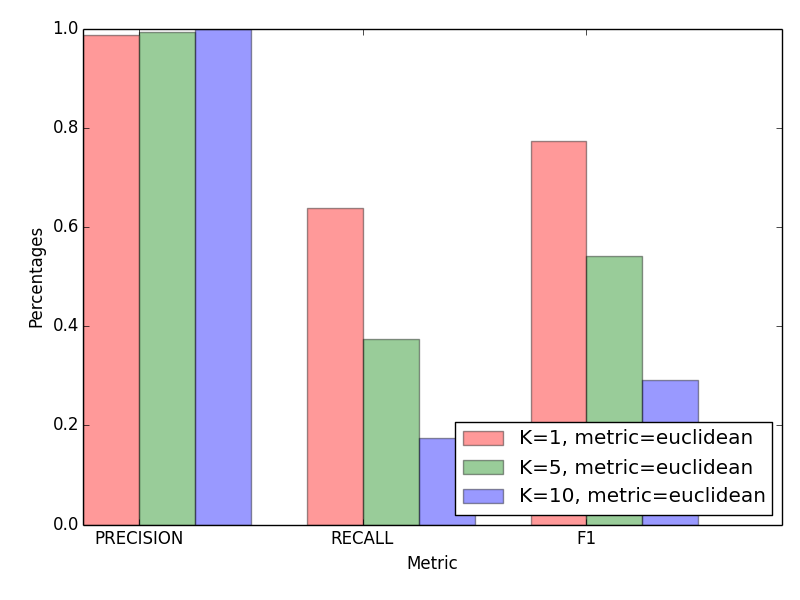
\includegraphics[height=3cm]{images/knear_tf_idf_euclidean}
		%\caption{}
	\end{subfigure}
	\begin{subfigure}{.3\textwidth}
		\centering
		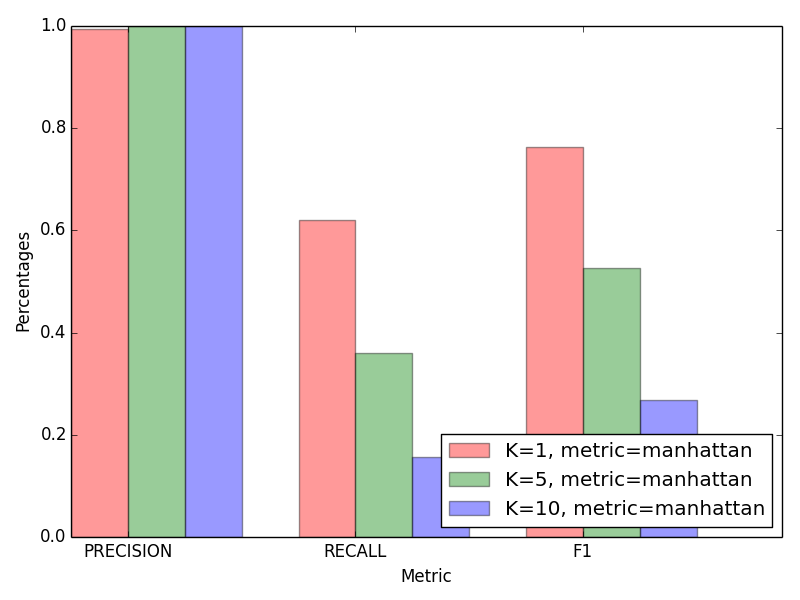
\includegraphics[height=3cm]{images/knear_tf_idf_manhattan}
		%\caption{}
	\end{subfigure}
	\begin{subfigure}{.3\textwidth}
		\centering
		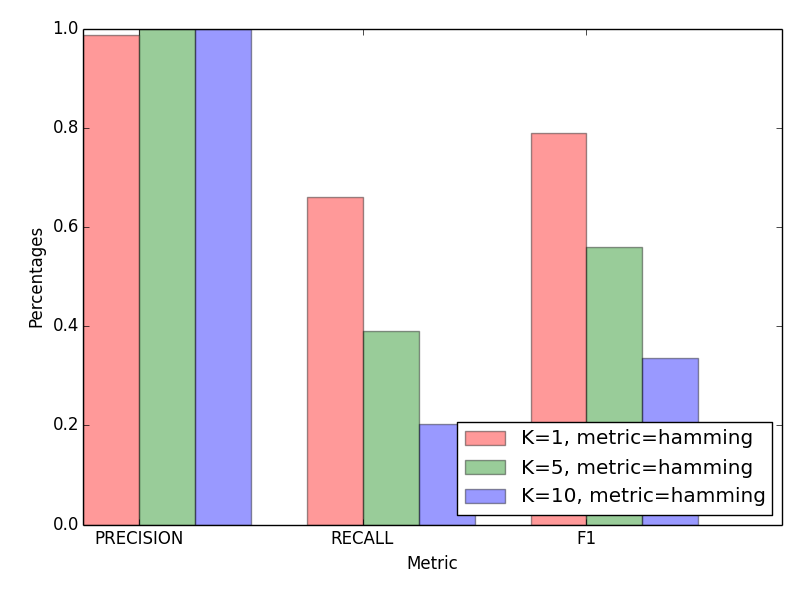
\includegraphics[height=3cm]{images/knear_tf_idf_hamming}
		%\caption{}
	\end{subfigure}
	\caption{Comparação de K-Nearest Neighbor com Term Frequency}
	\label{fig:knear_tf_idf}
\end{figure}

% GRAPHICS
%\begin{table}[ h ]
	\centering
	\resizebox{.8\textwidth}{!}{%
	\begin{tabular}{ | c | c | c | c | c | c | c |  }
		\hline
		Metric & K & Precision & Recall & F-Measure & Mn. Abs. Error & Mn. Sqr. Error  \\ \hline
		\multirow{4}{*}{Euclidean} 
 				& 1 & 0.99 & 0.70 & \textcolor{red}{0.82} & 0.041 $\pm$ 0.009 & 0.041 $\pm$ 0.009 \\ \cline{2-7}
				& 5 & 0.99 & 0.44 & 0.60 & 0.075 $\pm$ 0.013 & 0.075 $\pm$ 0.013 \\ \cline{2-7}
				& 10 & 1.00 & 0.26 & 0.41 & 0.0987 $\pm$ 0.0104 & 0.0987 $\pm$ 0.0104 \\ \cline{2-7}
				& 50 & 0.70 & 0.03 & 0.06 & 0.130 $\pm$ 0.004 & 0.130 $\pm$ 0.004 \\ \hline
		\multirow{4}{*}{Manhattan} 
 				& 1 & 0.99 & 0.68 & 0.81 & 0.044 $\pm$ 0.007 & 0.044 $\pm$ 0.007 \\ \cline{2-7}
				& 5 & 1.00 & 0.41 & 0.58 & 0.079 $\pm$ 0.009 & 0.079 $\pm$ 0.009 \\ \cline{2-7}
				& 10 & 1.00 & 0.22 & 0.36 & 0.105 $\pm$ 0.009 & 0.105 $\pm$ 0.009 \\ \cline{2-7}
				& 50 & 0.50 & 0.02 & 0.04 & 0.131 $\pm$ 0.003 & 0.131 $\pm$ 0.003 \\ \hline
		\multirow{4}{*}{Hamming} 
 				& 1 & 0.99 & 0.66 & 0.79 & 0.047 $\pm$ 0.007 & 0.047 $\pm$ 0.007 \\ \cline{2-7}
				& 5 & 1.00 & 0.39 & 0.56 & 0.082 $\pm$ 0.009 & 0.082 $\pm$ 0.009 \\ \cline{2-7}
				& 10 & 1.00 & 0.21 & 0.34 & 0.107 $\pm$ 0.006 & 0.107 $\pm$ 0.006 \\ \cline{2-7}
				& 50 & 0.50 & 0.02 & 0.04 & 0.131 $\pm$ 0.003 & 0.131 $\pm$ 0.003 \\ \hline
	\end{tabular}%
	}
	\caption{Comparação de K-Nearest Neighbor com Term Frequency}
	\label{tab:knear_comparison_term}
\end{table}
%\begin{figure}[H]
	\centering
	\begin{subfigure}{.3\textwidth}
		\centering
		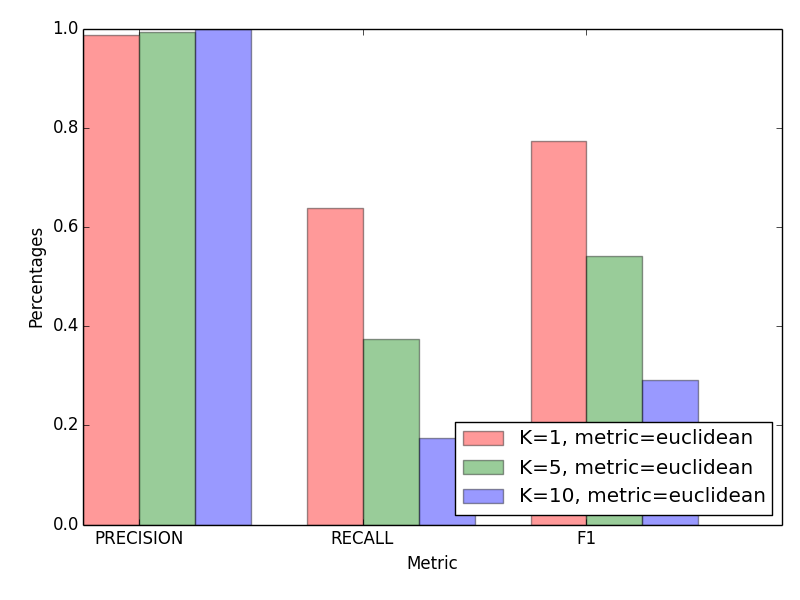
\includegraphics[height=3cm]{images/knear_tf_idf_euclidean}
		%\caption{}
	\end{subfigure}
	\begin{subfigure}{.3\textwidth}
		\centering
		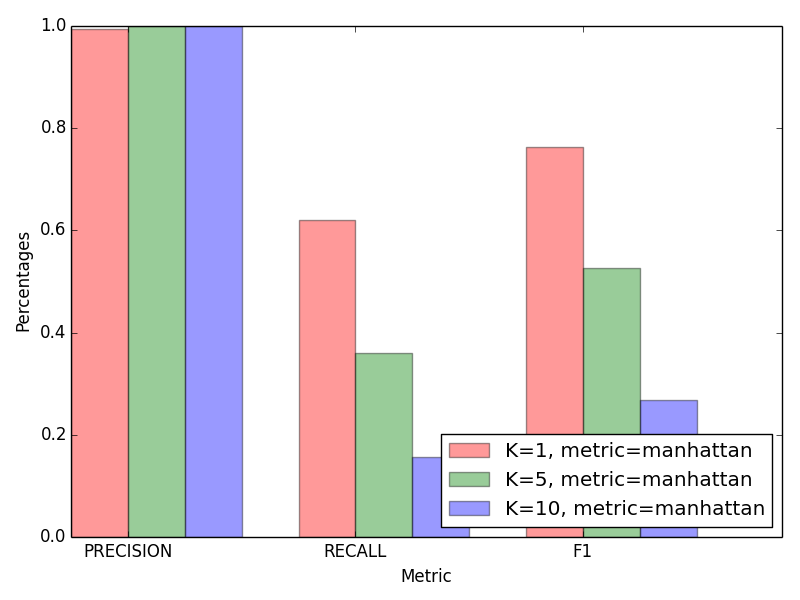
\includegraphics[height=3cm]{images/knear_tf_idf_manhattan}
		%\caption{}
	\end{subfigure}
	\begin{subfigure}{.3\textwidth}
		\centering
		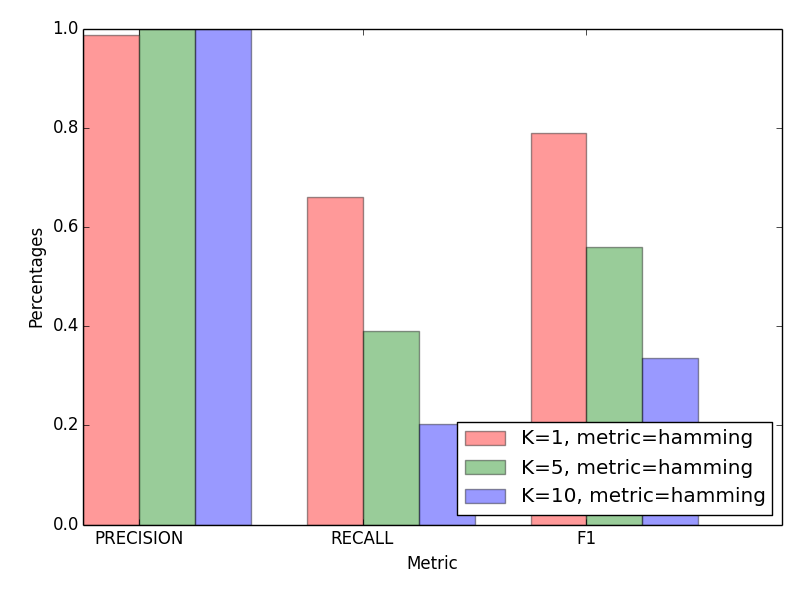
\includegraphics[height=3cm]{images/knear_tf_idf_hamming}
		%\caption{}
	\end{subfigure}
	\caption{Comparação de K-Nearest Neighbor com Term Frequency}
	\label{fig:knear_tf_idf}
\end{figure}